\documentclass[conference]{IEEEtran}
\usepackage{amsmath,booktabs,graphicx,cite,microtype}
\usepackage[hidelinks]{hyperref}
\begin{document}
\title{Published-Receiver Baselines and Perceptual Evaluation\\for Self-Calibrated Interference Cancellation}
\author{\IEEEauthorblockN{Experimental validation note}
\IEEEauthorblockA{19 September 2026}}
\maketitle
\begin{abstract}
This note documents a paired receiver comparison that distinguishes published
algorithms from internal calibration ablations. A fixed SwinJSCC representation
is decoded directly, with a CDDM receiver port, with the original ICDM receiver,
or with blind alternating calibration. Pixel error, learned perceptual distance,
and multiscale structural similarity are evaluated on the same reconstructions.
The study uses development data and is not an independent confirmation or a
reproduction of the complete systems' published performance numbers.
\end{abstract}

\section{Why These Baselines}
The scientific question concerns inference with a fixed transmitter, not a
comparison between differently trained image codecs. SwinJSCC~\cite{yang2025swinjscc}
therefore supplies the shared codec and a direct-decoding reference.
CDDM~\cite{wu2024cddm} tests whether a desired-signal prior and Gaussian
denoising suffice. ICDM~\cite{wu2026icdm} is the closest published receiver:
it separately models the desired signal and structured interference.
Global-energy and fixed-block-energy variants remain internal ablations;
they are not counted as separate external methods.

The CDDM comparison requires an explicit qualification. The original system
trains a denoiser and subsequently adapts its decoder. Here, its deterministic
denoising update is ported to the same pretrained DiT prior and frozen decoder
used by the interference-cancellation receivers. ICDM's own comparison also
uses a DiT-based CDDM, but with a different sampling budget. Our port uses the
prior's discrete training schedule and at most 40 uniformly respaced noise
predictions. It is denoted CDDM-RX throughout, rather than presented as a
complete reproduction of the original three-stage system.

Two information conditions are retained for CDDM-RX: thermal-noise power only
($N_0$), and true global noise-plus-interference power (oracle). ICDM retains its
published true-global-SINR amplitude and guidance lookup. SC-ICDM A4 receives
neither true SINR nor local interference powers. Thus, the oracle rows expose
their additional information; they are not described as blind competitors.

\section{Paired Protocol and Metrics}
The validation set consists of 64 sorted CelebA/CIFAR-10 image pairs, each
evaluated with two fixed channel seeds, six SINRs ($-7,-4,0,4,7,10$~dB), and
stationary, alternating, and burst interference. Noise SNR is 20~dB. Blocks
contain 64 complex symbols. All five receiver conditions see identical received
samples. The codec, desired-signal prior, and interference prior are frozen.
The desired images are $128\times128$ RGB; the encoder emits 1024 complex
symbols, giving a channel-use ratio of $1/48$ per RGB value. The stored codec
was trained using image MSE, not the LPIPS training objective of the ICDM
paper. These differences preclude copying numerical claims from that paper.

All images are clipped to $[0,1]$ before evaluation, without resizing or
quantization. For image $i$ with $D$ RGB values,
\begin{equation}
 e_i=D^{-1}\lVert\hat{\boldsymbol{s}}_i-\boldsymbol{s}_i\rVert^2,
 \qquad \mathrm{PSNR}_i=-10\log_{10}e_i.
\end{equation}
We average $e_i$ and $\mathrm{PSNR}_i$ separately. Taking the logarithm of the
dataset-average MSE would produce a different PSNR summary. These two metrics
describe the same pixel-error family rather than two independent advantages.

LPIPS uses the official VGG-based version 0.1 with images explicitly mapped
to $[-1,1]$; smaller values indicate better perceptual fidelity. MS-SSIM uses
four scales at this image resolution, an $11\times11$ Gaussian window with
$\sigma=1.5$, and the normalized first four published scale weights.
Each scale enters the product once; larger values indicate higher structural
similarity. The legacy local implementation repeated the last-scale factor,
so all methods are re-evaluated with a separately tested implementation.
The five-scale implementation agrees numerically with \texttt{pytorch-msssim};
the four-scale implementation also passes identity, batch-separation, and
analytic constant-image tests. Four-scale scores must not be compared directly
with unspecified five-scale scores from another study.

\section{Validation Results}
Table~\ref{tab:published-baselines} reports the complete validation run.  The
blind A4 receiver obtains the lowest arithmetic mean image MSE and LPIPS and
the highest mean MS-SSIM.  CDDM-RX with true global SINR obtains the highest
mean per-image PSNR, exceeding A4 by 1.011~dB.  This is not a numerical
inconsistency: PSNR is computed per image before averaging, whereas the MSE
column is the arithmetic mean of the per-image squared errors.  A small number
of difficult images therefore have substantially greater influence on mean
MSE than on mean PSNR.

\begin{table*}[t]
\centering
\caption{Paired receiver validation with a fixed SwinJSCC representation
($64$ image pairs, two channel seeds, six SINRs, and three interference
profiles; $2304$ matched conditions per receiver).  Oracle receivers know the
true global SINR; A4 does not.}
\label{tab:published-baselines}
\setlength{\tabcolsep}{7pt}
\begin{tabular}{lcccc}
\toprule
Receiver & PSNR (dB) $\uparrow$ & Image MSE $\downarrow$ & LPIPS-VGG $\downarrow$ & MS-SSIM $\uparrow$ \\
\midrule
SwinJSCC direct & 18.866 & 0.028305 & 0.4314 & 0.7067 \\
CDDM-RX ($N_0$ only) & 19.044 & 0.027870 & 0.4283 & 0.7101 \\
CDDM-RX (global-SINR oracle) & \textbf{21.583} & 0.019567 & 0.3425 & 0.8126 \\
ICDM (global-SINR oracle) & 19.147 & 0.025458 & 0.3760 & 0.7619 \\
SC-ICDM A4 (blind) & 20.571 & \textbf{0.015922} & \textbf{0.3407} & \textbf{0.8271} \\
\bottomrule
\end{tabular}
\end{table*}

Under exact pairing, A4 improves on direct SwinJSCC by 1.705~dB PSNR,
$0.012383$ MSE, $0.0907$ LPIPS, and $0.1204$ MS-SSIM on average.  Relative to
the global-SINR ICDM receiver, the corresponding changes are $+1.424$~dB,
$-0.009535$, $-0.0353$, and $+0.0652$.  By contrast, A4 has higher PSNR than
global-SINR CDDM-RX in only $26.7\%$ of the matched conditions.  Its better
overall MSE, LPIPS, and MS-SSIM means are driven by large improvements in the
most difficult conditions, rather than small improvements in most cases.

The conditional results locate that benefit.  Against global-SINR CDDM-RX,
A4 changes PSNR by $+2.098$ and $+0.403$~dB at $-7$ and $-4$~dB SINR,
respectively, while also improving all three remaining metrics.  From 0 to
10~dB, CDDM-RX is better in all four metrics.  A4 is likewise inferior for
stationary interference ($-2.446$~dB PSNR), where a global variance is an
adequate description.  For burst interference, A4 improves all four metrics,
including $+0.352$~dB PSNR, $-0.011719$ MSE, $-0.0749$ LPIPS, and $+0.0980$
MS-SSIM.  Alternating interference lies between these cases: A4 has
$0.940$~dB lower PSNR but slightly better mean MSE, LPIPS, and MS-SSIM.

These results support a conditional receiver rather than a universal
superiority claim: direct decoding at high SINR, global denoising when the
interference is approximately stationary, and local self-calibration for
strong nonstationary interference.  In particular, A4 loses 1.484~dB PSNR to
direct SwinJSCC at 10~dB SINR, so a high-SINR bypass is required by the data.


\begin{figure*}[t]
\centering
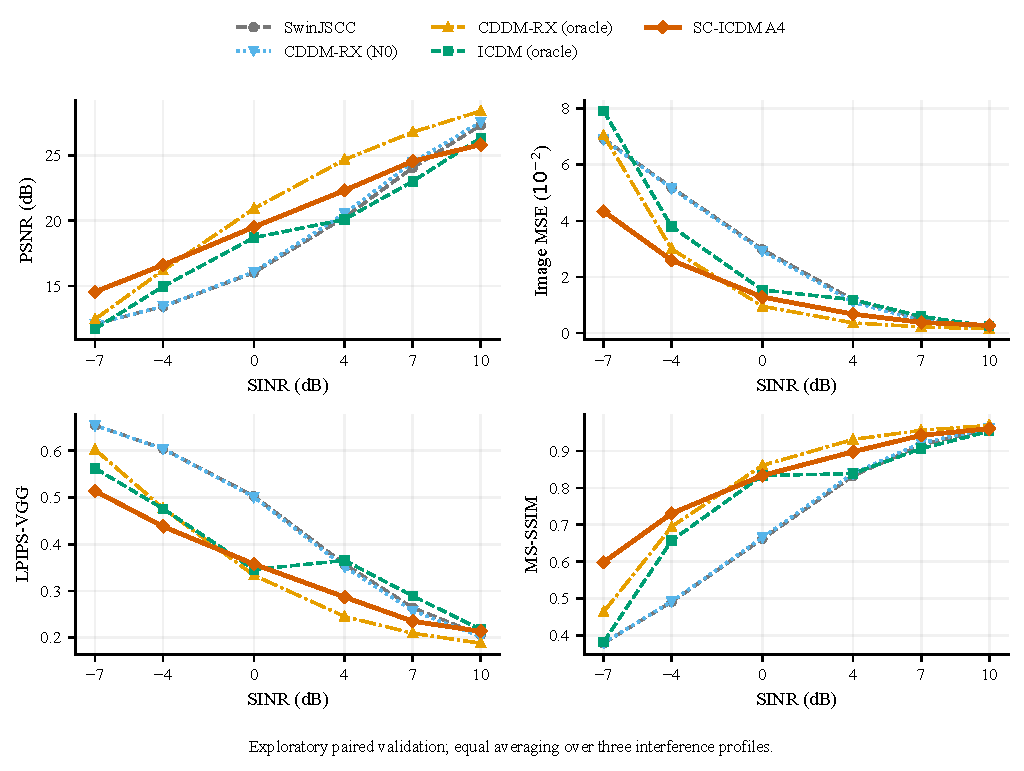
\includegraphics[width=\textwidth]{../../research/published_baselines_validation_v1/fig_metrics_overall.pdf}
\caption{Four quality metrics versus SINR, equally averaged over the three
interference profiles. Each point uses the same 64 image pairs and two channel
seeds. CDDM-RX is a shared-prior, frozen-decoder port; oracle methods know the
true global SINR. Profile-specific curves and individual records accompany
this note. The four plots must not be interpreted as four independent tests.}
\label{fig:metrics}
\end{figure*}

We report arithmetic means, paired mean differences, and the fraction of
matched conditions in which each receiver is better. No interval estimate or
dispersion summary is attached to this exploratory validation set. The
validation images were used in prior model selection, so no
independent-confirmation claim is made. Receiver timings are measured after
warm-up in the same
interleaved run on an RTX 4090, with batch size four. They include inference,
output normalization, and decoding, but exclude encoding and metric evaluation.
Another project's training process was detected on the host during execution;
the timing records are therefore diagnostic rather than an exclusive-hardware
efficiency comparison.

\section{Scope of the Evidence}
The comparison isolates receiver choices under a common representation and
records their differing side information. It does not establish superiority
over all published complete communication systems. CDDM's full training
pipeline, additional independent receiver families, fading, unknown block
boundaries, and a frozen held-out confirmation remain outside this run.
The existing 200-pair historical ablations must remain separate from these
64-pair validation results. Combining them into one larger sample would obscure
both the selection history and the evaluation protocol.

\bibliographystyle{IEEEtran}
\bibliography{references}
\end{document}
